% Figura 1 — Arquitetura do NOC Lite (C4 nivel container)
% Fonte: arquitetura_sistema.md (Dan), secao 1.2. Incluivel por \input ou \includegraphics.
\documentclass[tikz,border=4pt]{standalone}
\usepackage{tikz}
\usetikzlibrary{arrows.meta,positioning,calc}
\begin{document}
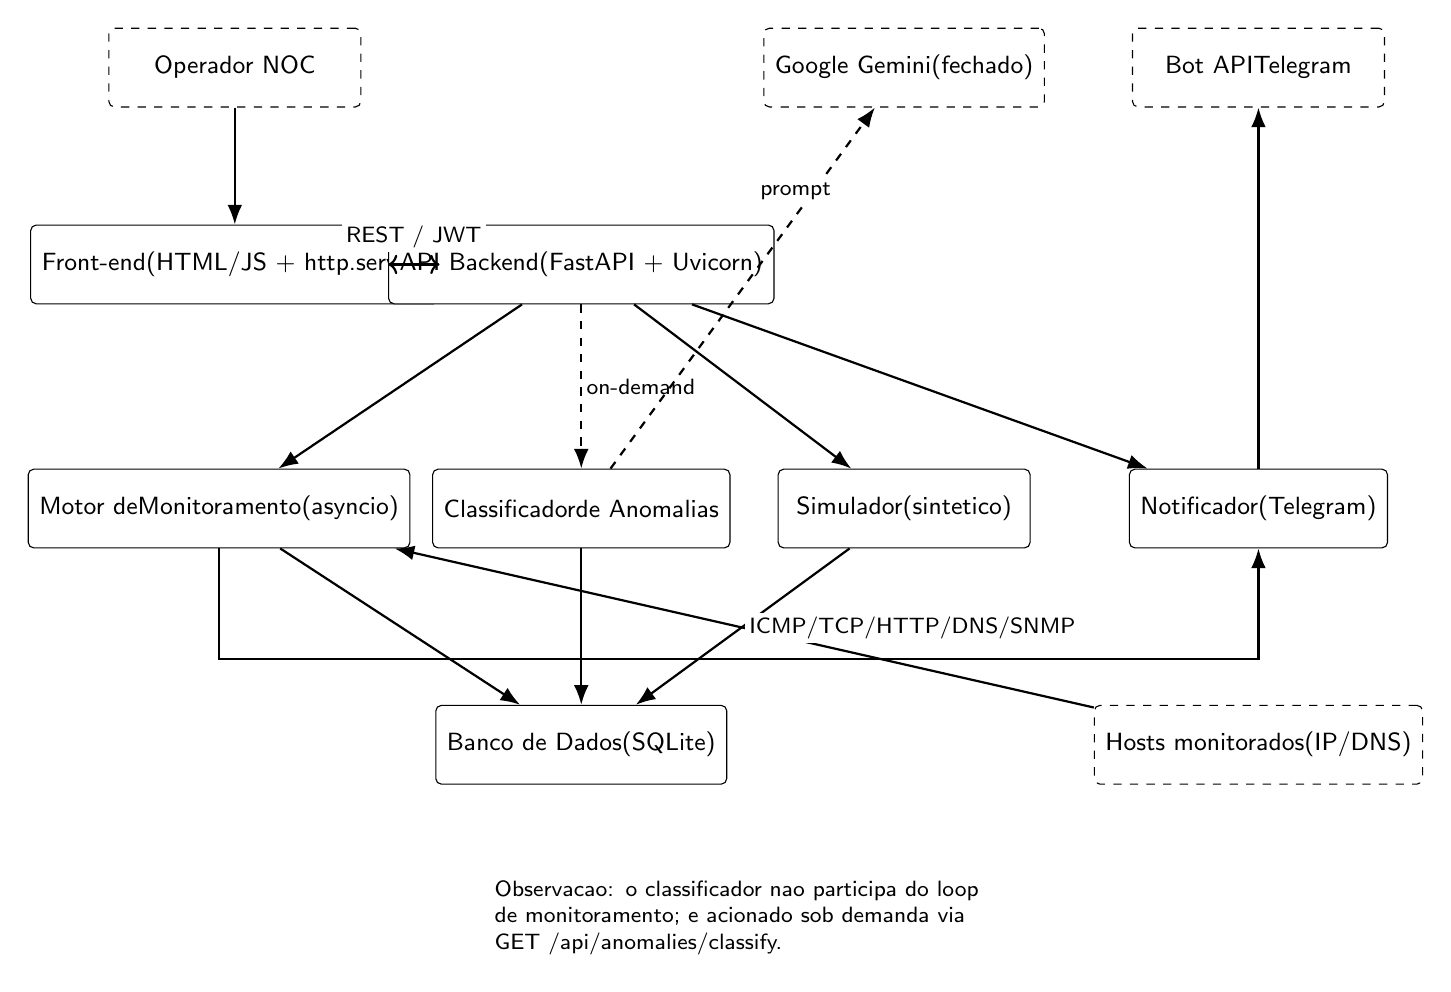
\begin{tikzpicture}[
    font=\sffamily\small,
    box/.style={rectangle, draw=black, rounded corners=2pt,
                minimum width=3.2cm, minimum height=1.0cm,
                text centered, fill=white, inner sep=4pt},
    ext/.style={rectangle, draw=black, dashed, rounded corners=2pt,
                minimum width=3.2cm, minimum height=1.0cm,
                text centered, fill=white, inner sep=4pt},
    arrow/.style={-{Latex[length=2.5mm]}, thick, draw=black},
    darrow/.style={-{Latex[length=2.5mm]}, thick, draw=black, dashed},
    lbl/.style={font=\sffamily\footnotesize, fill=white, inner sep=1.5pt},
  ]

  % --- Atores / sistemas externos (topo) ---
  \node[ext] (op)   at (2.0,11.2) {Operador NOC};
  \node[ext] (gem)  at (10.5,11.2){Google Gemini\\(fechado)};
  \node[ext] (tel)  at (15.0,11.2){Bot API\\Telegram};

  % --- Front-end / API ---
  \node[box] (fe)   at (2.0,8.7) {Front-end\\(HTML/JS + http.server)};
  \node[box, minimum width=3.6cm] (api)  at (6.4,8.7) {API Backend\\(FastAPI + Uvicorn)};

  % --- Contêineres centrais (linha do meio) ---
  \node[box] (mon)  at (1.8,5.6) {Motor de\\Monitoramento\\(asyncio)};
  \node[box] (cls)  at (6.4,5.6) {Classificador\\de Anomalias};
  \node[box] (sim)  at (10.5,5.6){Simulador\\(sintetico)};
  \node[box] (not)  at (15.0,5.6){Notificador\\(Telegram)};

  % --- Persistência / Hosts (base) ---
  \node[box] (db)   at (6.4,2.6) {Banco de Dados\\(SQLite)};
  \node[ext] (hosts)at (15.0,2.6){Hosts monitorados\\(IP/DNS)};

  % --- Fluxos ---
  \draw[arrow] (op)   -- (fe);
  \draw[<->,thick] (fe) -- (api) node[midway,above,yshift=4pt,lbl]{REST / JWT};
  \draw[arrow] (api)  -- (mon);
  \draw[darrow] (api) -- node[right,lbl]{on-demand} (cls);
  \draw[arrow] (api)  -- (sim);
  \draw[arrow] (api)  -- (not);

  \draw[arrow] (mon)  -- (db);
  \draw[arrow] (cls)  -- (db);
  \draw[arrow] (sim)  -- (db);
  % alertas: rota bem abaixo das caixas do meio (y=4.2)
  \draw[arrow] (mon)  |- ($(mon.south)+(0,-1.4)$) -| (not);
  \draw[darrow] (cls)  -- node[pos=0.7,above=4pt,lbl]{prompt} (gem);

  \draw[arrow] (hosts) -- node[right,lbl]{ICMP/TCP/\\HTTP/DNS/SNMP} (mon);
  \draw[arrow] (not)  -- (tel);

  % --- Anotação de escopo do classificador ---
  \node[font=\sffamily\footnotesize,text width=6.4cm,align=left]
        at (8.5,0.4) {Observacao: o classificador nao participa do loop de monitoramento; e acionado sob demanda via GET /api/anomalies/classify.};
\end{tikzpicture}
\end{document}
